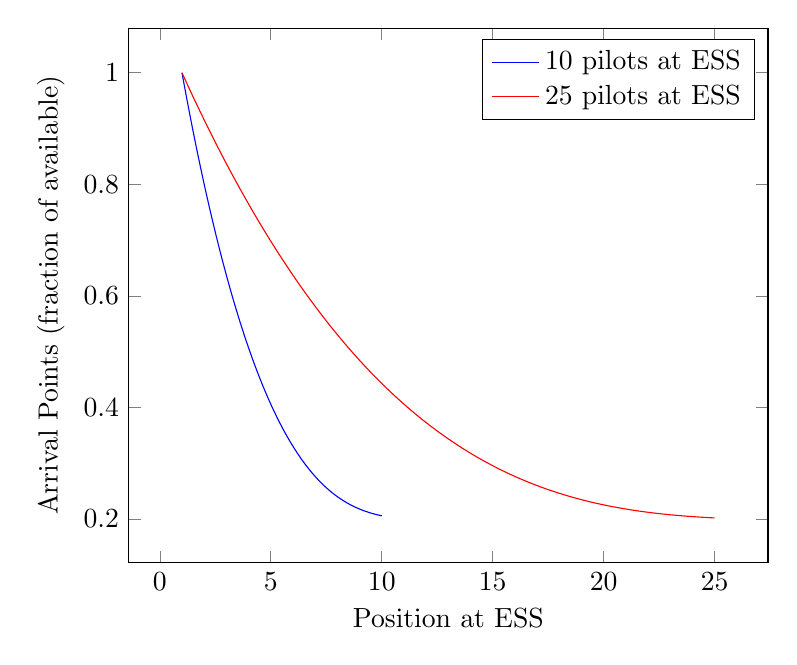
\begin{tikzpicture}
\begin{axis}[ xlabel=Position at ESS
            , ylabel=Arrival Points (fraction of available)
            , width=0.8\textwidth
            ]
    \addplot[ blue
            , domain=1:10
            , samples=100
            ]{0.2 + 0.037*(1 - (x - 1)/10) + 0.13*(1 - (x - 1)/10)^2 + 0.633*(1 - (x - 1)/10)^3};
    \addplot[ red
            , domain=1:25
            , samples=100
            ]{0.2 + 0.037*(1 - (x - 1)/25) + 0.13*(1 - (x - 1)/25)^2 + 0.633*(1 - (x - 1)/25)^3};
    \legend{10 pilots at ESS, 25 pilots at ESS} 
\end{axis}
\end{tikzpicture}
